\documentclass[12pt]{article}
\usepackage{amsmath}
%\usepackage{fullpage}
\usepackage[top=1in, bottom=1in, left=0.8in, right=1in]{geometry}
\usepackage{multicol}
\usepackage{wrapfig}
\usepackage{graphicx}
\usepackage{float}
\usepackage{listings}
\usepackage{enumerate}
\lstset{language=Java,
	basicstyle={\small\ttfamily},
	columns=flexible,
	belowskip=0mm}

\setlength{\columnsep}{0.1pc}

\title{ME573 Homework Set \# 9}
\author{Alexander Swenson -- \texttt{aaswenson@wisc.edu}}
\date{\today}
\begin{document}
	
	\maketitle
	
	\vspace{-0.3in}
	\noindent
	\rule{\linewidth}{0.4pt}
	
	\noindent
	

	
	%%%%%%%%%%%%%%%%%%%%%%%%%%%%%%%%%%%%%%%%%%%%%%%%%%%%%%%%%%%%%%%%%%%%%%%%%%%%%%%%
	
	\section{Problem 1}
	
	Show that for FTBS:
	
	\begin{equation}
	\frac{f_i^{n+1}-f_i^n}{\Delta t} + U \frac{f_i^n - f_{i-1}^n}{\Delta x} = 0
	\end{equation}
	
	\begin{equation}
	|\frac{A^{n+1}}{A^n}| ^2 = 1 - 2C_0(1-C_0)(1-cos\theta)
	\end{equation}
	
	From equation 1:
	
	\begin{equation}
	f_i^{n+1} = f_i^n - C_0(f_i^n - f_{i-1}^n)
	\end{equation}
	
	And from Von-Neumann Stability Analysis:
	
	\begin{equation}
		f_i^n = A^n e^{Ii\theta}
	\end{equation}
	
	Substitute 4 into 3:
	
	\begin{equation}
		A^{n+1}e^{Ii\theta} = A^ne^{Ii\theta} - C_0[A^ne^{Ii\theta} - A^ne^{I(i-1)\theta}]
	\end{equation}
	
	\begin{equation}
		\frac{A^{n+1}}{A^n}e^{Ii\theta} = e^{Ii\theta} - C_0[e^{Ii\theta} - e^{I(i-1)\theta}]
	\end{equation}
	
	\begin{equation}
		\frac{A^{n+1}}{A^n} = 1 - C_0[1 - e^{-I\theta}]	
	\end{equation}
	
	Which matches the Pozrikis's definition for $\frac{A^{n+1}}{A^n}$. Now we square the definition.
	
	\begin{equation}
		|\frac{A^{n+1}}{A^n}|^2 = -2C_0^2e^{i\theta} + C_0^2e^{2i\theta} + C_0^2 + 2C_0e^{i\theta}-2C_0 + 1
	\end{equation}
	
	\begin{equation}
		|\frac{A^{n+1}}{A^n}|^2 = C_0[-2C_0e^{i\theta} + C_0e^{2i\theta} + C_0 + 2e^{i\theta}-2] + 1
	\end{equation}
	
	\begin{equation}
		|\frac{A^{n+1}}{A^n}|^2 = 2C_0[-C_0e^{i\theta} + \frac{C_0e^{2i\theta}}{2} + \frac{C_0}{2} + e^{i\theta}-2] + 1
	\end{equation}
	
	\begin{equation}
		|\frac{A^{n+1}}{A^n}|^2 = 2C_0[-C_0(cos\theta + isin\theta) + \frac{C_0(cos(2\theta) + isin(2\theta)}{2} + \frac{C_0}{2} + (cos\theta + isin\theta)-2] + 1
	\end{equation}
	
	\begin{equation}
		|\frac{A^{n+1}}{A^n}|^2 = 2C_0[(1-C_0)(cos\theta + isin\theta) + \frac{C_0}{2}(cos(2\theta) + isin(2\theta) -1)] + 1
	\end{equation}
	
	\begin{equation}
		|\frac{A^{n+1}}{A^n}|^2 = (1-2C_0)[(1-C_0)(cos\theta + isin\theta) + \frac{C_0}{2}(cos(2\theta) + isin(2\theta))]
	\end{equation}
	
	The final step to reach Equation 2 is unclear.
		

	

	

	
	
	%%%%%%%%%%%%%%%%%%%%%%%%%%%%%%%%%%%%%%%%%%%%%%%%%%%%%%%%%%%%%%%%%%%%%%%%%%%%%%%%
	
		
	\section{Problem 2}
	
	\noindent Figure \ref{fig:ftcs_ftbs} displays results of the FTCS and FTBS schemes compared to the exact solution. This implementation of the scheme ($\Delta t$= 0.01 and $\Delta x$= 0.05) was stable ($C_0=0.628$)
	
		\begin{figure}[H]
			\centering
			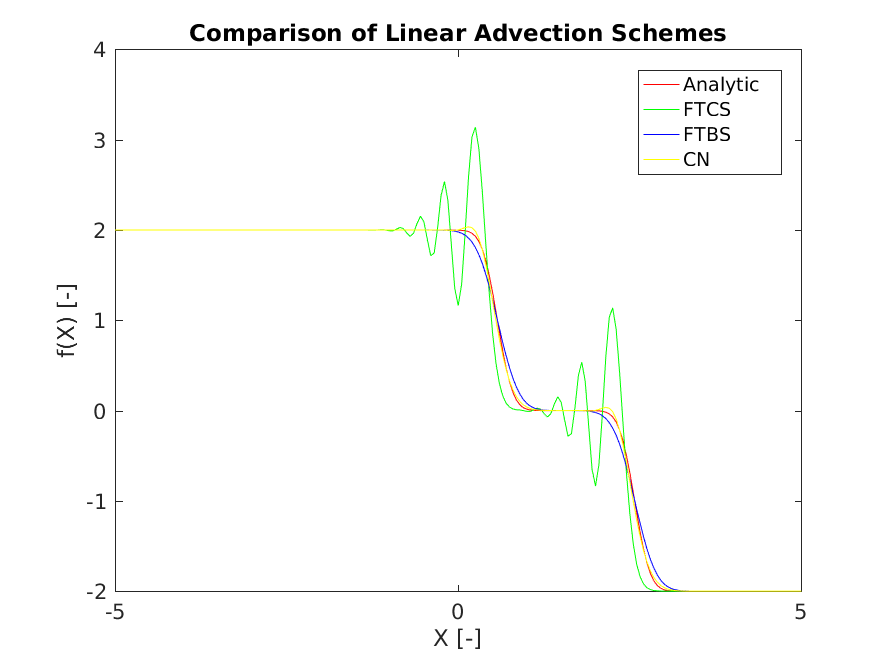
\includegraphics[height=3.75in]{ftcs_ftbs.png}
			\label{fig:ftcs_ftbs}
			\caption{}
		\end{figure}
		
	\noindent The FTBS scheme was re-implemented in an unstable condition ($\Delta t$= 0.02 and $\Delta x$= 0.025), the Courant number in this state is 2.51. Figure \ref{fig:ftbs_unstable} shows the results of this unstable solution.
	
	\begin{figure}[H]
		\centering
		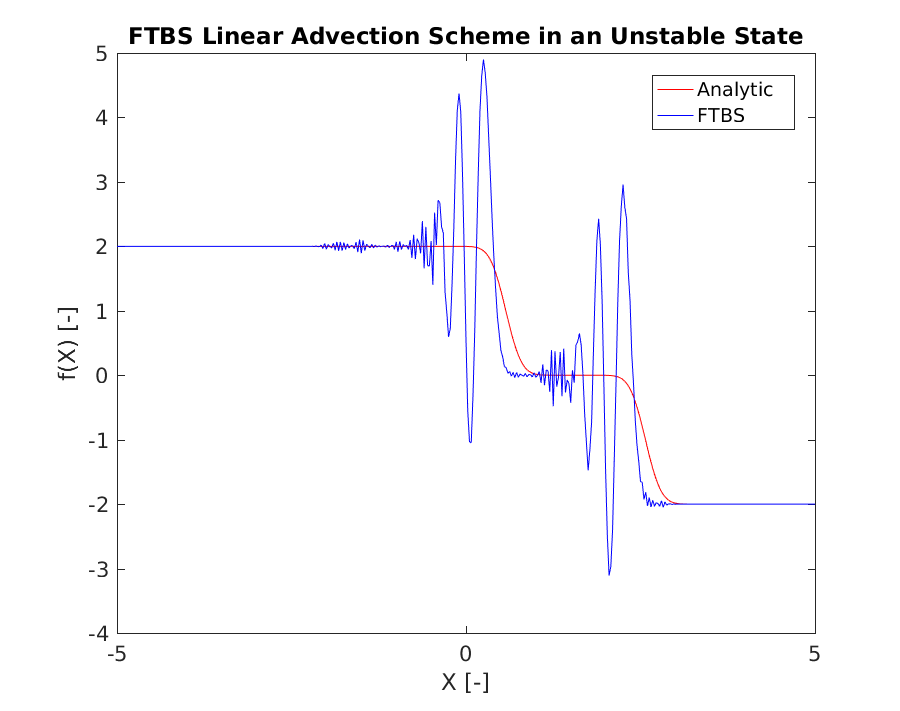
\includegraphics[height=3.75in]{ftbs_unstable.png}
		\label{fig:ftbs_unstable}
		\caption{}
	\end{figure}
	
	\section{Problem 3}
	
	Finally, the Crank-Nicolson Scheme was implemented to solve the same pure advection problem. Figure \ref{fig:ftbs_CN} shows the results of the CN approach compared to the FTBS scheme and Figure \ref{fig:ftbs_CN_error} shows the spatial error.
	
	\begin{figure}[H]
		\centering
		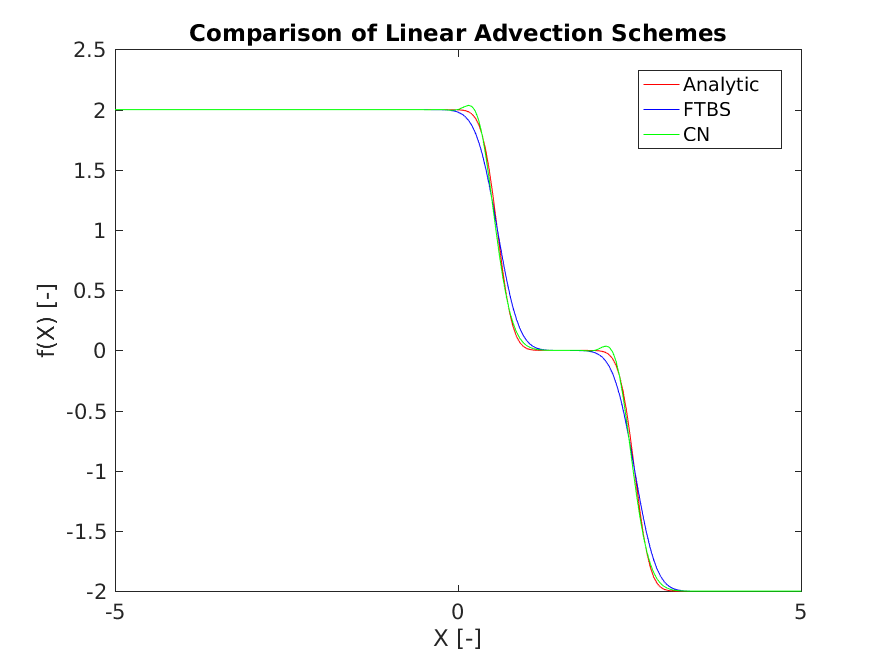
\includegraphics[height=3.75in]{ftbs_CN.png}
		\label{fig:ftbs_CN}
		\caption{}
	\end{figure}
	
	\begin{figure}[H]
		\centering
		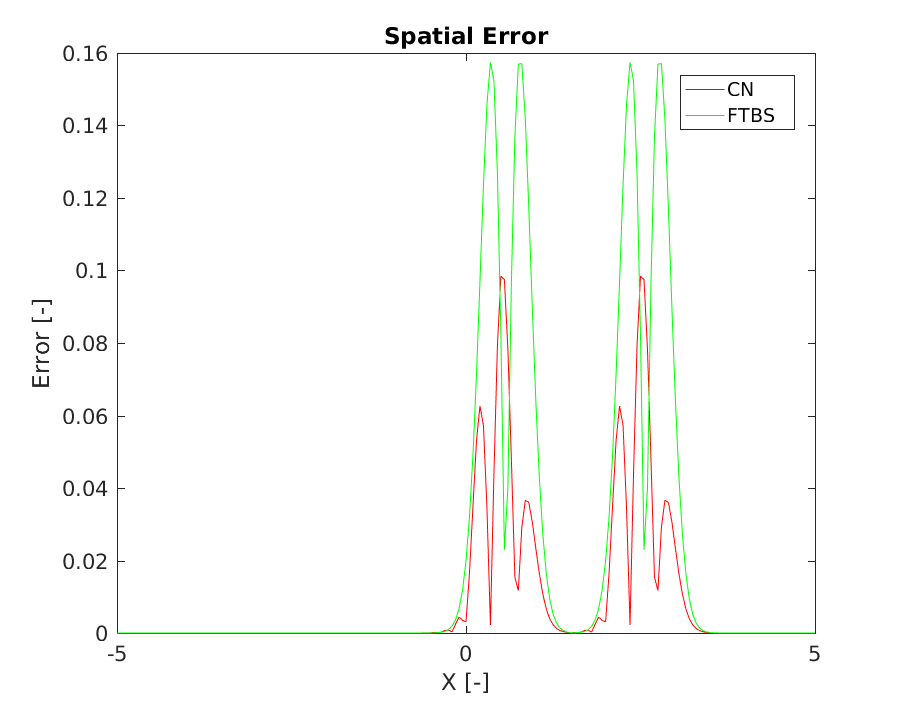
\includegraphics[height=3.75in]{ftbs_CN_error.png}
		\label{fig:ftbs_CN_error}
		\caption{}
	\end{figure}
	




%%%%%%%%%%%%%%%%%%%%%%%%%%%%%%%%%%%%%%%%%%%%%%%%%%%%%%%%%%%%%%%%%%%%%%%%%%%%%%%%

		
	
	
	
	
\end{document}
